\chapter{\color{oxfordblue} Theoretical Particle Physics}\label{chap-theory}
\ChapFrame

\textit{Particle Physics is the field of science dedicated to the study of the fundamental elements of matters and of their interactions. Nature at this scale is best represented by an intricate connexion between particles, the fundamental components of matter, and their interactions, themselves represented by particles. This framework is encapsulated into a mathematical foundation called quantum field theory. A major scientific achievement of the second half of the XX$^{\text{th}}$ century is the elaboration of the so-called Standard Model of Particle Physics, a unified patchwork of theories describing all known elementary particles and three of the four fundamental interactions affecting them. This chapter reviews relevant elements of the theory to contextualise the work presented in this thesis.}

\section{The Standard Model of Particle Physics}\label{Section:SM}
To date, the \gls{sm} has been the most successful theory in describing the constituents and the dynamics of matter \cite{SMphysics}. The \gls{sm} stands at the centre of theoretical particle physics, ellaborated by combining different successful theories of quantum mechanis and special relativity in the second part of the XX$^{th}$ century. These different exploits have led to a total of 55 Nobel Prizes. The \gls{sm} is often hailed as the most successful theory of science, with the unique ability to predict properties of the Universe to a staggering degree of precision: most famously, the anomalous magnetic dipole moment predictions is in agreement with measurements to up to 10 significant decimals \cite{PhysRevA.83.052122}. The \gls{sm} is expressed in the language of the dynamics of quantised fields, or \gls{qft}. These fields play two roles: describing matter itself (\textit{fermions}, such as the electron) and the different interactions (\textit{bosons}, such as the $W$ and the Higgs boson $H$) governing how this matter interacts under the electromagnetic, weak, and strong interactions. Particles are the results of local excitations of quantised fields that are defined as operator-values distributions over spacetime. Figure \ref{particlesSM} displays the fundamentals particles of the \gls{sm}. \\

\begin{figure}[!h]
    \centering
    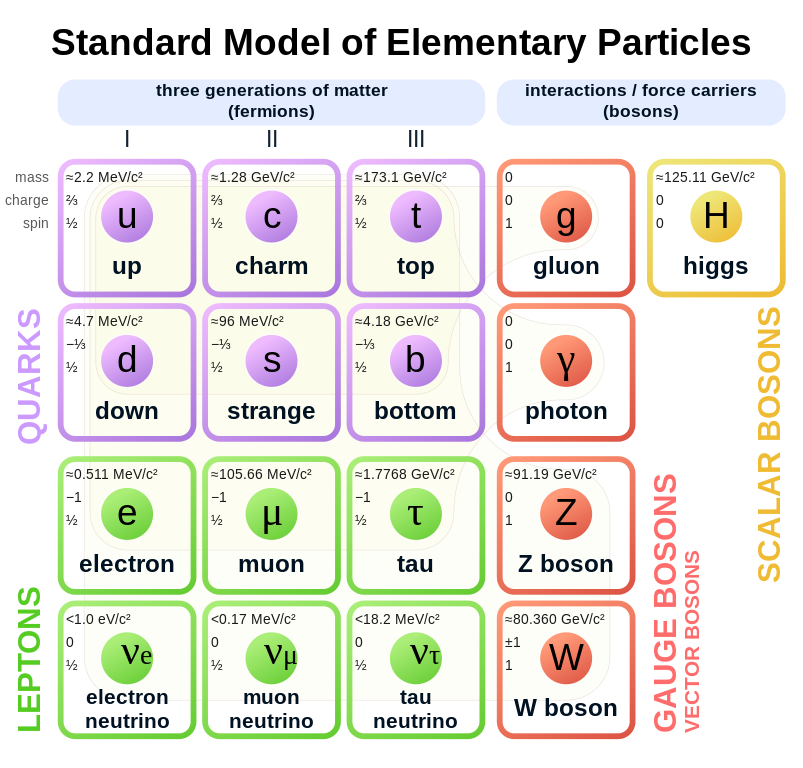
\includegraphics[width=0.8\textwidth]{Images/Theory/particlesSM.png} % TODO update to a more up to date. % TODO update the ref
    \caption[Particles in the SM]{Elementary particles of the Standard Model \cite{tableSMWiki}. Elementary fermions (quarks on top, lepton on the bottom) are listed in the three left columns and elementary bosons in the two right ones, the gauge bosons in the first column and the Higgs scalar boson in the last one. The mass, electrical charge, and spins of the particles are indicated.}
    \label{particlesSM}
\end{figure}

Particles are separated based on their intrinsic angular momentum or \textit{spin}, with half-spin particles following the Fermi-Dirac statistics called \textit{fermions}, and integer-spin particles called \textit{bosons} following the Bose-Einstein statistics. The elementary fermions are evenly split into 6 quarks and 6 leptons, with only the first generation of each being stable. The distinction between these two types stems from the different quantum numbers categorising them. Quarks carry a fractional electromagnetic charge as well as a colour charge making them sensitive to the strong interaction. On the contrary, leptons are colour-neutral and either have an electrical charge of -1$e^+$, in units of the anti-electron (positron) charge, or are neutral. The charged leptons include the electron $e^-$ - the lightest and only stable one -, the muon $\mu^-$, and the tau $\tau^-$. The neutral leptons are called neutrinos, with one neutrino $\nu_\ell$ associated per charged lepton $ell$, e.g., the electron-neutrino $\nu_e$. For the quarks, the electromagnetic charge is fractional, dividing them evenly between \textit{up}-type quarks with charge +$\frac{2}{3}$ consisting of the up $u$, charm $c$, and top $t$ flavours, and the \textit{down}-type quarks with charge -$\frac{1}{3}$ and the flavours down $d$, strange $s$, and bottom $b$. To every particle corresponds an \textit{anti}particle, with the same quantum numbers except for the electrical charge that changes sign. \\

The kinematics and dynamics of the fields representing the particles in the theory are expressed through a Lagrangian density $\mathcal{L}$, a spacetime discretisated element of the general Lagrangian. Symmetries of the Lagrangian density play an essential role as they define conserved quantities through Noether's theorem. The construction of the \gls{sm} Lagrangian id dictated by the expression of these symmetries to satisfy the experimentally observed conserved quantities, such as the electromagnetic charge. Two types of symmetries can be considered: global ones that are valid across spacetime and local ones, the so-called gauge symmetries valid for localised transformations. The \gls{sm} Lagrangian must satisfy the global Poincaré symmetry, encapsulating the symmetry required for special relativity, and a local non-Abelian $SU(3)_C \otimes SU(2)_L \otimes U(1)_Y$ gauge symmetry. Non-Abelian groups are such that their generators do not commute. The Lagrangian density of a field $\psi$ is a function of $\psi$ and its spacetime partial derivative $\partial_{\mu} \psi$, where $\mu$ indexes the time and space dimenions in the 4-vector formalism. The full \gls{sm} Lagrangian $\mathcal{L}_{\text{SM}}$ can be decomposed into 4 terms:
\begin{equation}\label{eq-SMGlobal}
    \mathcal{L}_{\text{SM}} = \mathcal{L}_{\text{EW}} + \mathcal{L}_{\text{QCD}} + \mathcal{L}_{\text{Higgs}} + \mathcal{L}_{\text{Yukawa}}.
\end{equation}
These different terms represent different effects encoded within the unified framework of the \gls{sm}. Three of the four known interactions of nature are encapuslated in the \gls{sm}: the strong, the electromagnetic, and the weak forces, with the gravitational force considered aside due to the weakness of its influence at sub-atomic scales. The mediators of the three included interactions are the gauge bosons, spin 1 particles with different properties arising from the nature of the interaction they carry. The electromagnetic and weak force have been successfully unified as a single \gls{ew} interaction, while the theory of the strong force is \gls{qcd}. One essential element in the \gls{sm} is the so-called Higgs interaction, a special force through which some gauge bosons acquire mass. This Higgs interaction is underpinned by a Higgs field, an excitation of which is called a Higgs boson $H$. Interactions between the Higgs field and quark can be introduced to assign masses to the latter through Yukawa couplings. The latter part of this thesis is dedicated to a measurement of such couplings to $b$- and $c$-quarks. The different interactions and their respective gauge bosons are further reviewed in this chapter.

\subsection{Quantum Electrodynamics}\label{subsec-QED}
\glsfirst{qed} is the theory underpinning the behaviour of free fermions and their electromagnetic interactions, for which the gauge carried are the photons. Fermions are represented by a Dirac spinor field $\psi(x)$ defined over spacetime $x$. The Dirac equation of quantum mechanics is a first order partial derivative equation modelling the free dynamics of such a spin-$\frac{1}{2}$ fermion with:
\begin{equation}\label{eq-dirac}
    (i\gamma^{\mu} \partial_{\mu} - m) \psi = 0,
\end{equation}
where $\gamma^{\mu}$ are the Dirac $\gamma$-matrices generalising the Pauli spin matrices to spacetime dimension, and the Einstein notation is adopted, summing over indices repeated as covariant and contravariant. For clarity, any contraction $\gamma^{\mu} \partial_{\mu}$ is denoted as $\cancel{\partial}$. A Lagragian density can be constructed to result in the dynamics described by Equation \ref{eq-dirac} through application of Euler-Lagrange:
\begin{equation}\label{eq-diracLag}
   \mathcal{L}_{\text{Dirac}} = \bar{\psi} (i \cancel{\partial}- m) \psi,
\end{equation}
Such a Lagrangian models the free dynamics of any spin-$\frac{1}{2}$ fermion, such as an electron $e^-$. Electrons have a $q = -1$ charge that is conserved by every known interactions. This conservations must be the result of a symmetry: the Dirac Lagrangian must be made invariant under a local gauge $U(1)$ transformation:
\begin{equation}\label{eq-GaugeU1}
    \psi \rightarrow \psi' = e^{-iq\alpha(x)} \psi ,
\end{equation}
which corresponds to a rotation in the complex spacetime by a phase $q\alpha(x)$. For the Lagrangian of Equation \ref{eq-diracLag} to satisfy this symmetry, the partial derivative $\partial_{\mu}$ must be replaced by the \textit{gauge covriant derivative $D_{\mu}$}:
\begin{equation}\label{eq-CoDerU1}
    \partial_{\mu} \rightarrow \partial_{\mu} + iqA_{\mu},
\end{equation}
where a new vector field $A\mu$ is introduced and required to transform under the $U(1)$ symmetry as $A_{\mu} \rightarrow A'_{\mu} = A_{\mu} + \partial_{\mu} \alpha(x)$. The elegance of this approach is the possibility to give this fauge field $A_{\mu}$ its own dynamic, modifying the Lagrangian of Equation \ref{eq-diracLag} into the \gls{qed} Lagrangian: \[ \mathcal{L}_{\text{QED}} = \bar{\psi} (i \cancel{\partial}- m) \psi + q \bar{\psi} \cancel{A} \psi - \frac{1}{4} F_{\mu\nu} F^{\mu\nu} \]
\begin{equation}
    \mathcal{L}_{\text{QED}} = \bar{\psi} (i \cancel{D}- m) \psi - \frac{1}{4} F_{\mu\nu} F^{\mu\nu}
\end{equation}
where $F_{\mu\nu} = \partial_{\mu} A_\nu - \partial_\nu A_{\mu} $ is the electromagnetic field tensor. The last term introduces a kinetic term for the gauge field and the interaction between the fermion $\psi$ and the gauge field $A$ is represented by the term combining them. In the present case, the charge $q$ is the conserved quantity of the gauge symmetry, which required the introduction of a new gauge field $A_\mu$ that can be interpreted as the photon field and given the dynamic of the electromagnetic interaction through $F_{\mu\nu}$. Fermionic fields can be introduced in this approach for the different known fermions, $\psi_e$, $\psi_{\mu}$, $\psi_u$, $\psi_c$, etc. Their interactions with $A_\mu$ defining each time a unique conserved electromagnetic charge $q_e$, $q_{\mu}$, $q_u$, $q_c$, etc.  This procedure is however general: the gauge invariance of a Lagrangian introduces a spin-1 gauge vector boson. The required $U(1)$ invariance forbids the presence of mass terms of the form $m^2 A^{\mu} A_{\mu}$, seemingly condemning the gauge bosons to be massless. 

\subsection{Electroweak Sector}
The weak force is described by two massive gauge vector bosons: the $W^{\pm}$ of mass $m_W \approx 80.4$ GeV\footnote{The unit system adopted throughtout this thesis is to set the speed of light in vacuum $c$ at 1, leading to masses expressed in GeV. To convert to mass units, one simply needs to divide by the standard unit $c^2$.} and the $Z^0$ of mass $m_Z \approx 91.2$ GeV. This apparent contradiction with the massless requirements of a $U(1)$ symmetry is elegantly solved by the Brout-Englert-Higgs mechanism \cite{Englert:1964et,  PhysRevLett.13.508}. This mechanism, described in the next section, is applied to a joint expression of the electromagnetic and weak forces known as \glsfirst{ew} theory in the Glashow-Weinberg-Salam (GWS) model \cite{GLASHOW1961579, PhysRevLett.19.1264, Salam:1968rm}. The fundamental symmetry group the theory is built upon is the non-Abelian $SU(2)_L \otimes U(1)_Y$, where $SU(2)_L$ is the weak isospin and $U(1)_Y$ the weak hypercharge. A local $SU(2)$ transformation acts as:
\begin{equation}\label{eq-GaugeSU2}
    \psi \rightarrow \psi' = e^{i g \alpha^a(x) T^a } \psi,
\end{equation}
where $T^a = \sigma^a / 2$ are the generators of the $SU(2)_L$ group, built from the $\sigma^a$ Pauli matrices ($a = 1, 2, 3)$. Each generator corresponds to a gauge field. The gauge field linked to $SU(2)_L$ leads to covariant derivative, simularly to Equation \ref{eq-GaugeSU2}, to ensure gauge invariance as expressed by
\begin{equation}\label{eq-GaugeSU2}
   D_{\mu}  = \partial_{\mu} + igT_a W_{\mu}^a,
\end{equation}
with three gauge fields $W_{\mu}^1$, $W_{\mu}^2$, $W_{\mu}^3$ with interaction strength $g$. The particularity of the weak interaction is that the charged current interactions described by the symmetry group $SU(2)_L$ only apply to left-handed $L$ particles states and not the right-handed $R$. Consequently, fermionic fields are decomposed into \[\psi = \psi_L + \psi_R\] with left-and right-handed particles represented by isospin doublets. The weak isospin $I_W$ charge of left-handed particles is $I_W = 1/2$, with a third component $I_W^3 = \pm  1/2$. For the right-handed part, $I_W = 0$ with $I_W^3 = 0$, decoupling it from the gauge bosons $W_{\mu}^a$. Physically, the observed weak charge current interaction corresponding to the $W^{\pm}$ bosons are the linear combinations of gauge fields:
\begin{equation}
    W_{\mu}^{\pm} = \frac{1}{\sqrt{2}} \left(W_{\mu}^{1} \mp W_{\mu}^{2} \right)
\end{equation}
These $W$ bosons only couple to left-handed particles, but an experimentally observed $Z$ boson couples to both left- and right-handed particles. This represented by the additional $U(1)_Y$ symmetry of the weak interaction in the \gls{sm}, with weak hypercharge $Y$, coupling $g'$, and an additional gauge field $B_{\mu}$. The weak hypercharge is \[Y = 2 (Q - I_W^3),\] with $Q$ the electromagnetic charge. The total covariant derivative of the electroweak sector of the \gls{sm} is therefore expressed by the GSM model as 
\begin{equation}\label{eq-GaugeEW}
    D_{\mu}  = \partial_{\mu} + ig T_a W_{\mu}^a + ig' \frac{Y}{2} B_{\mu}. % TODO should these be the g and g
\end{equation}
where $W_{\mu}^a$ and $B_{\mu}$ are respectively the $SU(2)_L$ and $U(1)_Y$ gauge bosons. The GSM model re-expresses the electromagnetic photonic field $A_\mu$ and the $Z$-boson field $Z_{\mu}$ as a linear combination of $B_{\mu}$ and $W_{\mu}^3$ depending on the \textit{weak mixing angle} $\theta_W$, a fundamental parameter of the \gls{sm} such that:
\begin{equation}\label{eq-weakmixangle}
    \cos\theta_W = \frac{g}{\sqrt{g^2 +g'^2}}.
\end{equation}
This establishes a connexion between the coupling strengths of the weak interaction and the electromagnetic interaction coupling $e$ as \[e = g \sin \theta_W = g' \sin\theta_W \cos\theta_W.\] The intrinsic strength of the weak interactions is indeed of similar ordar to that of the electromagnetic interaction but is weak in apparance due to its gauge bosons being massive. The weak force is the only known fundamental interaction to violate parity conservation. Neutrinos can only interact throught the weak force, which can itself only apply to left-handed particles. As a result, there are no right-handed neutrinos in the \gls{sm}. \\

A significant achievement of modern particle physics is the unification of interactions that are perceived as different at low-energies. The problem of the measured mass of the vector gauge bosons remains. Additionaly, the split of fermionic fields into a left- and right-handed componets lead the mass terms to violate the gauge invariance. Both issues are resolved by the mechanisn of the Brout-Englert-Higgs and Yukawa interactions, introduced in the next sections.

\subsection{The Brout-Englert-Higgs Mechanism}
The Brout-Englert-Higgs mechanism, abbreviated $BEH$ henceforth, offers a solution to introduce mass terms to the gauge fields $W_{\mu}^{\pm}$ and $Z_{\mu}$ \cite{Englert:1964et,  PhysRevLett.13.508}. It introduces a new scalar Higgs field, permeating the Universe. The field is mathematically defined as a weak isospin doublet, with a neutral component $\phi^0$ and a charged one $\phi^+$. They are jointly expressed as complex scalar field with 4 degrees of freedom:
\begin{equation}
\phi = \begin{pmatrix}
    \phi^+\\ 
    \phi^0
\end{pmatrix} = \frac{1}{2} \begin{pmatrix}
    \phi_1 + i\phi_2 \\ 
    \phi_3 + i\phi_4
\end{pmatrix}
\end{equation}
This complex scalar field is made to interact with the electroweak gauge fields as 
\begin{equation}\label{eq-HiggsLag}
    \mathcal{L_{\text{Higgs}}} = (D_{\mu}\phi)^{\dagger} (D^{\mu}\phi) - V(\phi),
 \end{equation}
where the first term described the kinetic of the $\phi$ and the second term is the Higgs potential energy:
\begin{equation}\label{eq-HiggsLag}
 V(\phi) = - \mu^2  \phi^{\dagger} \phi + \lambda (\phi^{\dagger} \phi)^2.
\end{equation}
where the expression of this potential is constrained by the need for the theory to be renormalisable. Two scalars constants govern the Higgs potential: $\mu$ and $\lambda$ describing, respectively, the quadratic and quartic interaction of the complex Higgs field $\phi$. The former manifests the interaction with the gauge bosons, while the latter introduces self-interactions. The minimum of this potential corresponds to the vacuum state. The requirement that the vacuum be stable demands $\lambda > 0$. For a positive $\mu^2 > 0$, a degenerate minimum is found at field values such that
\begin{equation}\label{eq-HiggsLag}
    \phi^{\dagger} \phi  = \frac{1}{2} (\phi_1^2 + \phi_2^2 + \phi_3^2 + \phi_4^2) = \frac{- \mu^2}{2\lambda} = \frac{v^2}{2}
\end{equation}
introducing in the last equality the so-called \textit{vacuum expectation value} $v = \sqrt{\frac{|\mu^2|}{\lambda}}$ of the field $\phi$. This infinite degeneracy of the Higgs potential minimum states underlines a special $SU(2)$ symmetry such that $\phi^{\dagger} \phi = v^2/2$. Through \textit{spontaneous symmetry breaking}, the BEH mechanism crumbles this degeneracy into one single vacuum state, typically chosen by setting the components $\phi_1 = \phi_2 = \phi_4 = 0$ and $\phi_3 = v$ so that the vacuum expactation is simply
\begin{equation}
\langle0|\phi|0 \rangle = \frac{1}{\sqrt{2}} \begin{pmatrix}
        0\\ 
        v
    \end{pmatrix}.
\end{equation}
The breaking of the symmetry enforces \[ SU(2)_L \otimes U(1)_Y \rightarrow U(1)_Q,\] with the final vacuum state correctly set as chargeless. Expanding the full field dynamic around the chosen vacuum state with a particular gauge choice to absord unphysical Goldstone fields into the vector fields called \textit{unitarity gauge} \cite{PhysRevD.7.1068}, the expansion can be simplified to 
\begin{equation}
    \phi = \frac{1}{\sqrt{2}} \begin{pmatrix}
            0\\ 
            v + h(x)
        \end{pmatrix},
\end{equation}
where $h$ is the real neutral Higgs scalar field. Introducing this expression into the Higgs Lagrangian of Equation~\ref{eq-HiggsLag} gives
\begin{equation}\label{eq-fullHiggs}
    \begin{split}
        \mathcal{L}_{\text{Higgs}} = & \,\frac{1}{2} (\partial_\mu h)(\partial^\mu h) + \frac{\mu^2}{2}(v+h)^2  - \frac{\lambda}{16}(v+h)^4 \\
        &+ \frac{1}{4} g^2 (W_{\mu}^+W^{\mu-})(v+h)^2 + \frac{g^2_W + {g'}^2}{8}(Z_{\mu}Z^{\mu})(v+h)^2 
    \end{split}
\end{equation}
where one can clearly identify mass terms for the physical gauge fields $W_{\mu}^{\pm}$ and $Z_\mu$ in the last line, but not for $A_{\mu}$ as required from observations that photons are massless. The vector gauge bosons masses are:
\begin{equation}
    m_W = \frac{v}{2} g , \, m_Z = \frac{v}{2}\sqrt{g^2 +g'^2} 
\end{equation}
or equivalenty expressing the mass of the $Z$-boson in terms of the $W$-boson mass \[m_Z = \frac{m_W}{\cos\theta_W}.\] The Higgs field is massive\footnote{This requires to isolate the terms in $h^2$ in Equation \ref{eq-fullHiggs}.} with mass \[m_H = \sqrt{2|\mu^2|}.\]
The BEH mechanism elegantly assigns mass to the gauge vector boson, with the photon remaining massless and the addition of the Higgs boson $H$ as a massive elementary particle. Furthermore, the introduction of the related Higgs field permits the expression of mass terms for the fermions in the standard model, as explained in Section~\ref{subset-yukint} on Yukawa interactions. 

\subsection{Quantum Chromodynamics}
The strong interaction is described by the theory of \textit{\glsfirst{qcd}}, underpinned by an $SU(3)_C$ symmetry with conserved quantum number called \textit{colour}. The only particles having a colour charge in the \gls{sm} are quarks and gluons $g$, the gauge mediators of the strong interactions. There are three colour charges typically labelled \textit{red}, \textit{blue}, and \textit{green}, each coming into its direct or anti-colour (e.g., anti-red). Quarks carry one such charge and gluons two. Similarly to the electroweak sector, the symmetry leads to a covariant derivative under the $SU(3)_C$ group of
\begin{equation}\label{eq-GaugeQCD}
    D_{\mu}  = \partial_{\mu} + ig_s \lambda_a G_{\mu}^a. % TODO should these be the g and g
\end{equation}
where the coupling constant $g_s$ of the strong interaction is often re-expressed as $\alpha_s = \frac{g_s}{4\pi}$, and the generator of the $SU(3)_C$ group are the set of eight $\lambda_a$ Gell-Mann matrices. The gauge field introduced here are the $G_{\mu}^a$ corresponding to the associate mediator of the strong field: the gluons $g$. Gluons carry 2 colour charges, leading to the 8 Gell-Mann matrices $\lambda^a$ and 8 gauge vector fields $G_{\mu}^a$. The generators of the $SU(3)_C$ group do not commutate: \[ [\lambda^a, \lambda^b] = i f^{abc} \lambda^c,\] where $f^{abc}$ are the $SU(3)_C$ structure constants.  Similarly to the electromagnetic strength tensor, strength tensors are built from the gluon fields as \[G_{\mu\nu}^a = \partial_{\mu} G_{\nu}^a   - \partial_{\nu} G_{\mu}^a - g_s f^{abc} G_{\mu}^b G_{\nu}^c.\]
This leads to a total \gls{qcd} Lagrangian of:
\begin{equation}\label{eq-QCDLag}
    \mathcal{L}_{\text{QCD}} = -\frac{1}{4} G_{\mu\nu}^a G^{\mu\nu}_a + \sum_{k} \bar{\psi}_k (i \cancel{D} - m_k) \psi_k,
\end{equation}
where $\psi_k$ are the six quarks fields, one per flavour, transforming as an $SU(3)_C$ triplet with one component per colour quantum number. Cubic and quartir terms in the gluon gauge fields $G_{\mu}^a$ are included, introducing self interaction of gluons. The non-commutation of the $SU(3)_C$ generators means the $SU(3)_C$ part of the \gls{sm} is non-Abelian group, and therefore a case of a Yang-Mills theory requiring this self-interacting gauge fields \cite{PhysRev.96.191}. \\

Like every coupling constant, $\alpha_s$ varies with energy. At low energies, the interaction is so strong that perturbative calculation breaks and the behaviour of \textit{colour confinement} is observed: any attempt to isolate a quark requires so much energy that a quark-antiquark pair is spontaneously produced. The strength of this interaction explains it short propagation distance despite the fact its gluonic mediatiors are massless. At higher energies $\sim 100$ GeV, asympotic freedom and perturbative calculations are possible thanks to the smallness of the coupling strength. This typically requires higher-order corrections for calculation to converge, with some terms, such as quark self-energy loops, diverging to infinity. This type of diverge is  called \textit{ultraviolet divergence}, and it is fixed by renormalising fields and parameters so that the divergence are absorbed away. This correction requires two parameters to arbitrarily define the scale of the process: the \textit{renormalisation scale} $\mu_R$ and \textit{factorisation scale} $\mu_F$ \cite{collins2004factorization}. The former is introduced to deal with ultraviolet divergences in the running of $\alpha_s$. The latter addresses the so-called \textit{infrared divergences} due to massless particles radiating further massless particles at low-energies by entering the parton distribution and fragmentation functions, introduced latter in this chapter.\\

Quarks must combine to form colour-less aggregate of matters called hadrons, with either a 2-quark system combining a quark and an antiquark into a \textit{meson}, or a 3-quark system forming a \textit{baryon} of which the proton ($uud$, $q_p = +1$) and the neutrons ($udd$, $q_n = 0$) are prime examples. The content of hadrons are called partons. The process leading to the neutralisation of the colour-charge of an asymptotically freed quark is called \textit{hadronisation}.\\

\subsection{Yukawa Interactions}\label{subset-yukint}
In the \gls{qcd} Lagrangian of Equation~\ref{eq-QCDLag}, the introduction of the mass terms for the quarks breaks the gauge invariance of the theory to $SU(2)_L \otimes U(1)_Y$ and must be therefore further modified. The masses of all fermions can however be included in the \gls{sm} by introducing so-called Yukawa interactions between the Higgs and fermionic fields. Such terms are expressed as the following Lagrangian:
\begin{equation}\label{eq-YukLag}
    \mathcal{L}_{\text{Yukawa}} = - \frac{1}{\sqrt{2}} \sum_{f} 
    y_f \bar{\psi}_f (v + h) \psi_f,
\end{equation}
where $\psi_f$ are the fermionic fields and the fundamental \textit{Yukawa coupling} parameters $y_f = \sqrt{2} \frac{m_f}{v}$ for each flavour of fermion $f$ are introduced as coupling strengths. Picking the $v$ component in the sum in parenthesis gives a clear mass term to the fermion, with the $h$ terms leading to Higgs-fermion interactions. The vacuum expectation value plays the role of a mass scale setting, with Yukawa coupling refining the specific strength for each fermionic species. For the quark sector, a futher correction is required as the weak interaction eigenstate basis is different from the mass basis in which physical particles are detected. The transformation from the mass eigenstates basis is specified by the complex unitary \textit{\gls{ckm} matrix} \cite{Tanabashi:2018oca}:
\begin{equation}
    V_{CKM} = \begin{pmatrix}
            V_{ud} & V_{us} & V_{ub}\\ 
            V_{cd} & V_{cs} & V_{cb}\\ 
            V_{td} & V_{ts} & V_{tb}\\ 
        \end{pmatrix},
\end{equation}
where the probability of a transition $p \rightarrow q$ is given by the magnitude $|V_{pq}|^2$ of the associated element. Through this quark mixing matrix, weak charged currents interaction allows for flavour-changing processes through charged currents interactions. The matrix is almost diagonal, hence transitions between quarks of the same generation are preferred (e.g., $t \rightarrow b$ preferred over $t \rightarrow d$).

\section{Experimental Higgs Phenomenology}
The experimental process to observe the Higgs bosons at the \gls{lhc} is to collide two proton beams head-on, as described in Chapter~\ref{chapter-ATLAS}. The accelerator is primarily designed to achieve these measurements, targeting different production and decay channels. Protons are composite particules (hadrons) and, at high energies, the main \textit{hard-scattering} interaction is beteen components of the protons called \textit{partons}. These partons are primarily the \textit{valence} quarks ($uud$ for a proton) but also contribution from \textit{sea} quarks, as well as gluons and photons present within the hadron due to quantum interactions. In a $pp$ collision, two interacting partons $ab$ from within the protons undergo the main event $ab \rightarrow X$, with the activity from the rest of the protons assigned to the so-called \textit{\gls{ue}}. The cross-section for the global process $pp \rightarrow X$ is expressed using the factorisation theorem \cite{collins2004factorization} as 
\begin{equation}
\sigma_{pp\rightarrow X} = \sum_{a,b} \int_0^1 dx_a \int_0^1 dx_b f_a(x_a, \mu_F) f_b(x_b, \mu_F) \int d\sigma_{ab\rightarrow X}\left(x_aP_a, x_bP_b, \mu_R, \mu_F \right),
\end{equation}
where $f_i(x_i, \mu_F)$ is the \textit{\gls{pdf}} giving the probability for the parton $i$ to undergo a hard scattering with momentum $p_i = x_i P_i$, where $x_i$ is the fraction of the proton momentum $P_i$, $\mu_F$ is the previously introduced factorisation scale, as the \gls{pdf} depend on the energy scale of the underlying process. The interaction is effectively split into two steps: picking up the interacting partons and their fraction of momentum, then considering the main $ab \rightarrow X$ event.\\

As introduces in the previous section, the Higgs couples to particles proportionally to their measured mass, which influences its production and decay modes. The leading order production modes of the Higgs boson are schematised in Figure \ref{fig:prodH}. At the \gls{lhc} with a centre of mass energy $\sqrt{s} = 13$ TeV and a Higgs boson mass $m_H = 125$ GeV, the main processes presented are by decreasing cross-sections: 
\begin{itemize}[leftmargin=*] % TODO check values % TODO check for qqH
    \item \textit{Gluon-gluon fusion $ggF$}: two gluons fuse into a quark loop with a radiated Higgs boson: $pp \rightarrow H$. The quarks in the loop must couple to the Higgs, hence top $t$-quarks are preferred, followed by bottom $b$-quarks. The cross-section for this process is $\sigma_{ggF} = 48.6 \pm 2.4$ pb \cite{LHCHiggsCrossSectionWorkingGroup:2016ypw}. This process is favoured thanks the large contributions of gluons to the protonic \gls{pdf}s.
    \item \textit{Vector boson fusion $VBF$}: two off-shell vector bosons $V$ ($W$ or $Z$) radiated from partonic quarks fuse to form a Higgs $pp \rightarrow qqH$, with cross-section $\sigma_{VBF} = 3.77 \pm 0.09$ pb \cite{LHCHiggsCrossSectionWorkingGroup:2016ypw}. The quarks leave a characteristic twin forward jets in the event.
    \item \textit{Associated production with a vector boson $VH$}: the Higgs boson is produced in association with a vector boson $V$ ($W$ or $Z$): $pp \rightarrow VH$. This process is studied in greater detail in Chapter~\ref{}, dedicated to an analysis of Higgs decaying to $b$- or $c$-quarks from this production mode. It has a cross-section of $\sigma_{VH} = 2.24 \pm 0.14$ pb \cite{LHCHiggsCrossSectionWorkingGroup:2016ypw}. Leptonic decays of the associated vector boson give clean event signatures.
    \item \textit{Associated production with a quark pair $q\bar{q}H$}: an ``open quark loop'' is produced from a pair of partonic gluons, with a Higgs radiated $pp \rightarrow q\bar{q}H$. The dominating contributions come from the $t\bar{t}H$ associated production with cross-section $\sigma_{VH} = 0.51 \pm 0.04$ pb, followed by the $b\bar{b}H$ \cite{LHCHiggsCrossSectionWorkingGroup:2016ypw}.
\end{itemize}

\begin{figure}[h!]
    \center
    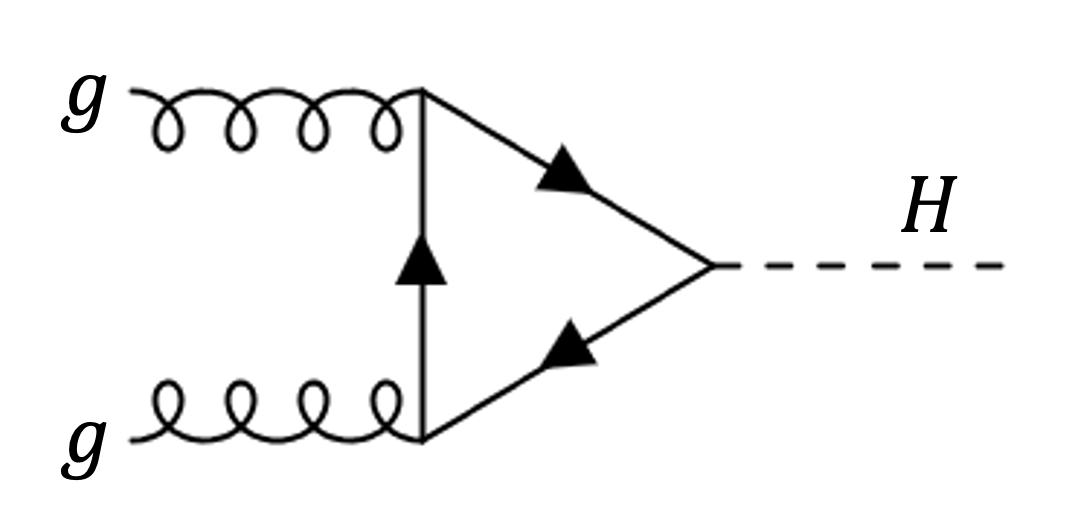
\includegraphics[width=0.24\textwidth]{Images/Theory/ggH.png}
    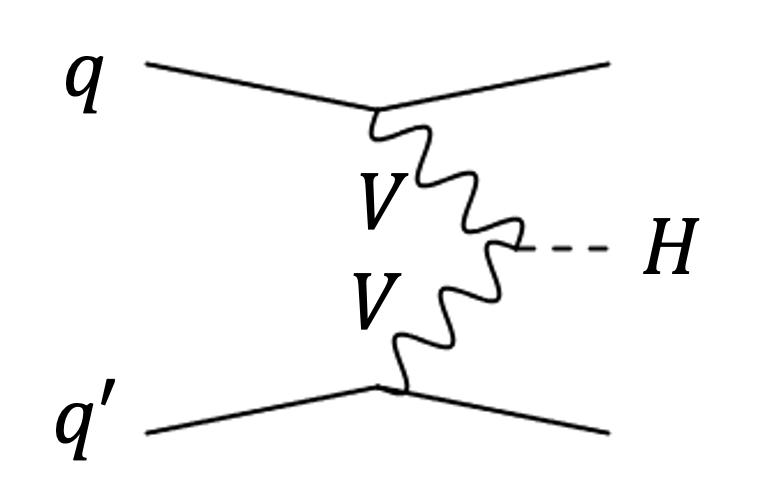
\includegraphics[width=0.24\textwidth]{Images/Theory/vvH.png}
    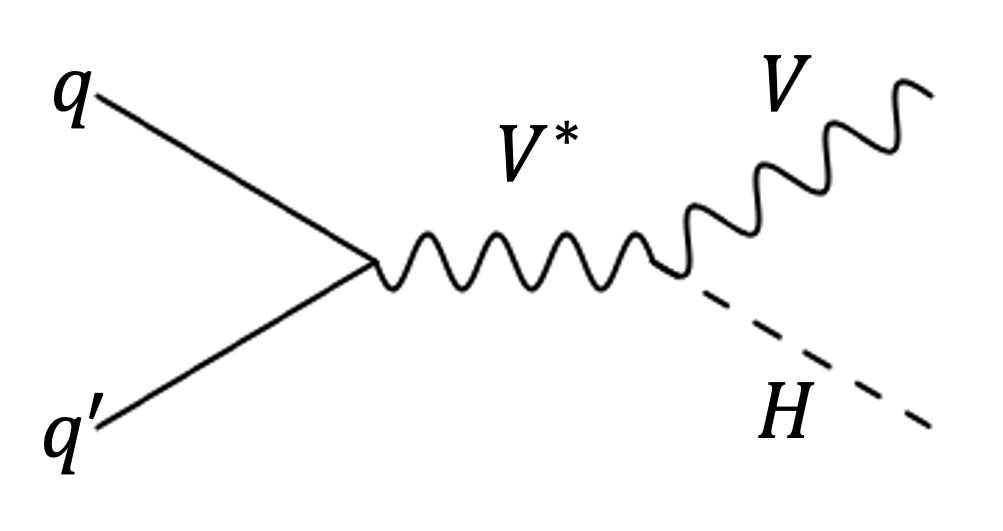
\includegraphics[width=0.24\textwidth]{Images/Theory/vh.png}
    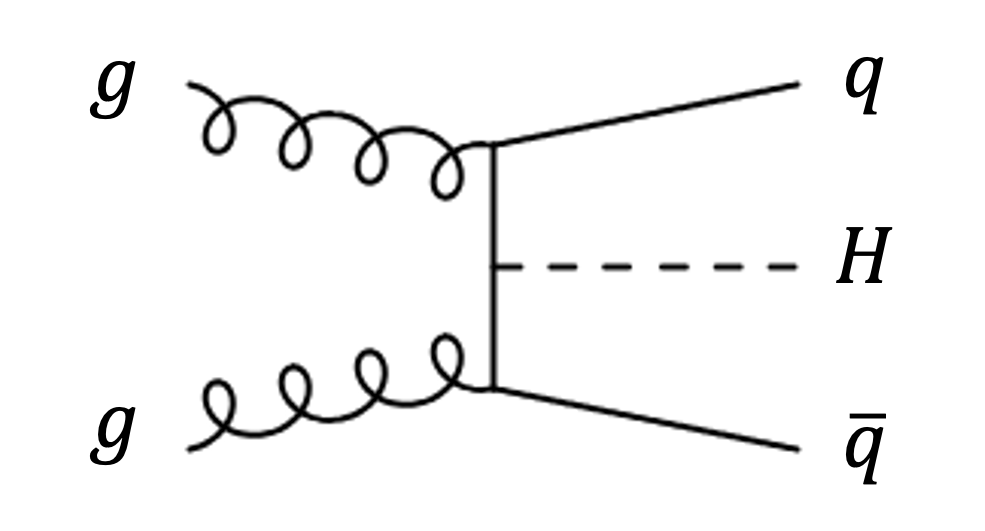
\includegraphics[width=0.24\textwidth]{Images/Theory/qqH.png}
    \caption{The leading order Feynman diagrams for Higgs production at the LHC, from left to right: gluon-gluon fusion ($ggF$), vector boson $V$ fusion ($VBF$), associated production with a vector boson ($VH$), and associated production with a $q\bar{q}$ pair ($q\bar{q}H$).}
    \label{fig:prodH}
\end{figure}

The dependency of the Higgs boson production from proton-proton collisions at $\sqrt{s} = 13$ TeV are represented in the left of Figure~\ref{fig:prodHcross} as a function of the Higgs boson mass $m_H$. The total width of the \gls{sm} Higgs boson is $\Gamma_H = 4$ MeV, implying a short lifetime of $\tau_H ~ 10^{-22}$ $s$ and restricting measurement to its decay products. The decay branching ratios are displayed in the right of the figure, with decays to heavier particles favoured due to the proportionality of the Higgs coupling strength to the mass. Decays to the massless gluons $g$ and photons $\gamma$ are possible thanks to intermediate quark loops, similarly to $ggF$. Relative decay rates are quantified by their branching ratio $BR$ as
\begin{equation}
    BR(H \rightarrow X) = \frac{\Gamma(H\rightarrow X)}{\Gamma_H}
\end{equation},
where the total Higgs width $\Gamma_H$ is the sum of all partial decay width $\Gamma(H\rightarrow X)$, for all possible $X$. The right of Figure~\ref{fig:prodHcross} displays the \gls{sm} Higgs branching ratio at $\sqrt{s} = 13$ TeV. The most likely Higgs decay mode is to a pair $b\bar{b}$ ($BR \approx 58$ \%), followed by the decay to a $WW$ pair ($BR \approx 21$ \%), and the $c\bar{c}$ decay branching ratio is 2.9\%. All the decay branching ratios are displayed in the right of the figure, with decays to heavier particles favoured due to the proportionality of the Higgs coupling strength to the mass. \\

\begin{figure}[h!]
    \center
    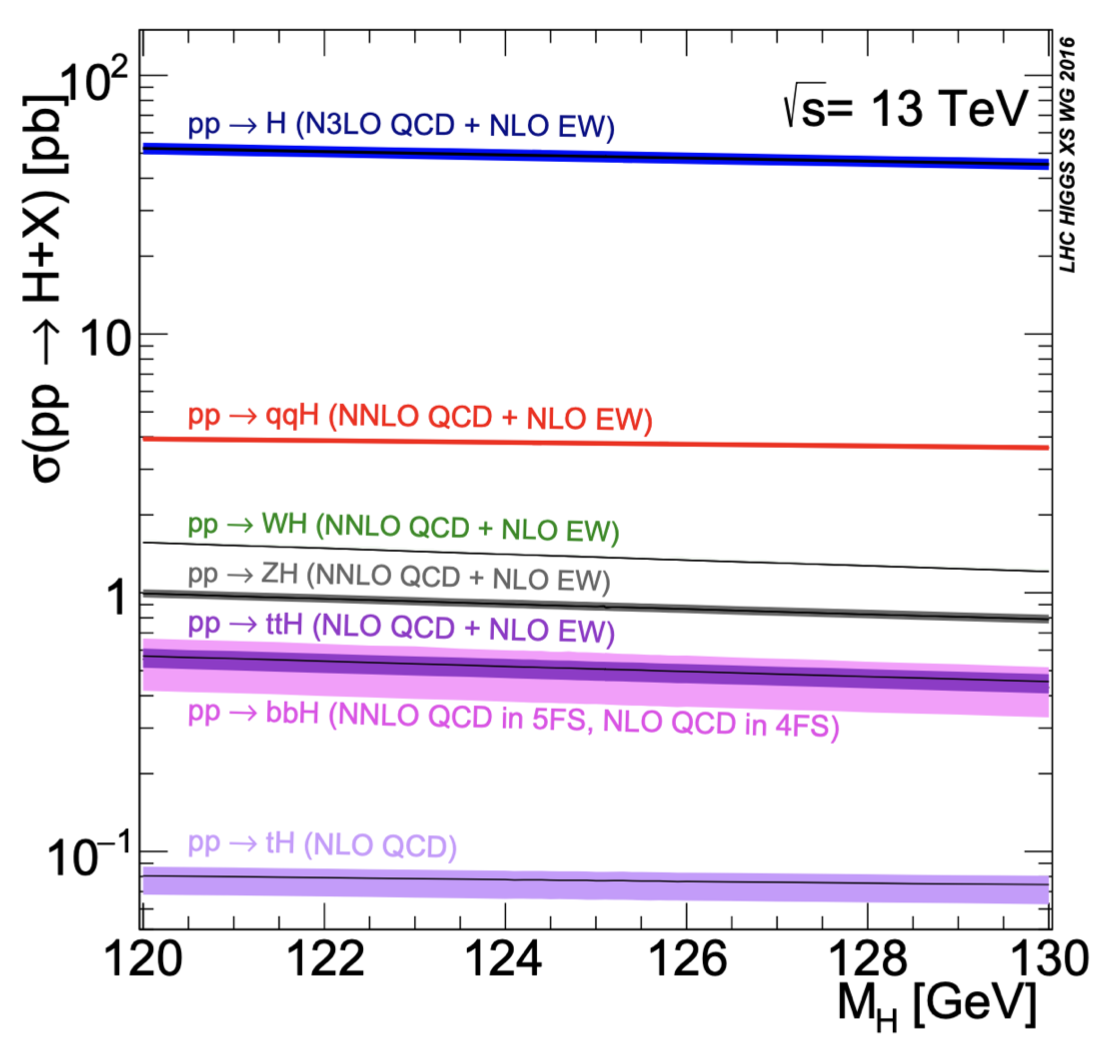
\includegraphics[width=0.48\textwidth]{Images/Theory/prodHiggs.png}
    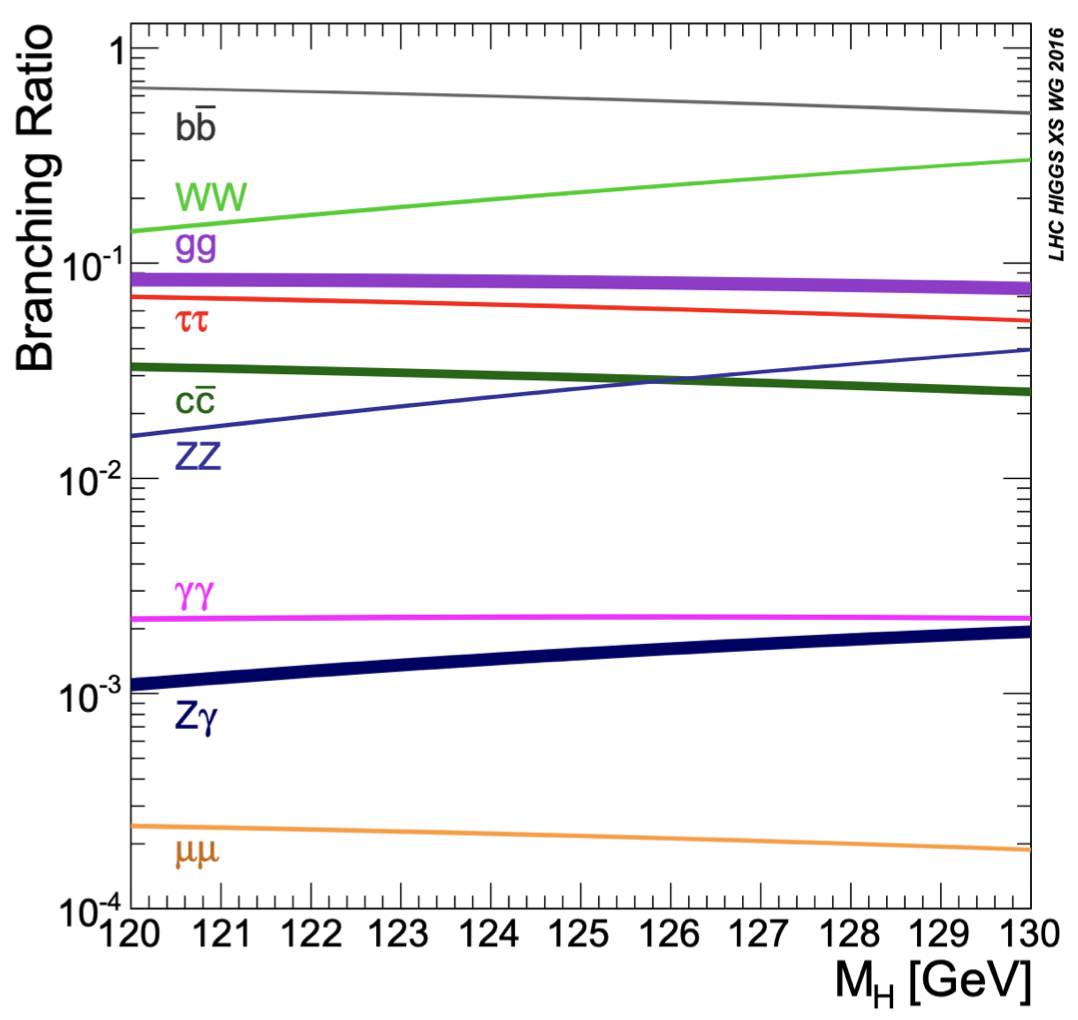
\includegraphics[width=0.48\textwidth]{Images/Theory/decayHiggs.png}
    \caption{The Standard Model production cross-sections from proton-proton collisions (left) and decay branching ratio (right) of the Higgs boson as a function of $m_H$, at $\sqrt{s} = 13$ TeV, from \cite{LHCHiggsCrossSectionWorkingGroup:2016ypw}.}
    \label{fig:prodHcross}
\end{figure}
\begin{figure}[h!]
    \hspace{-0.48cm}
    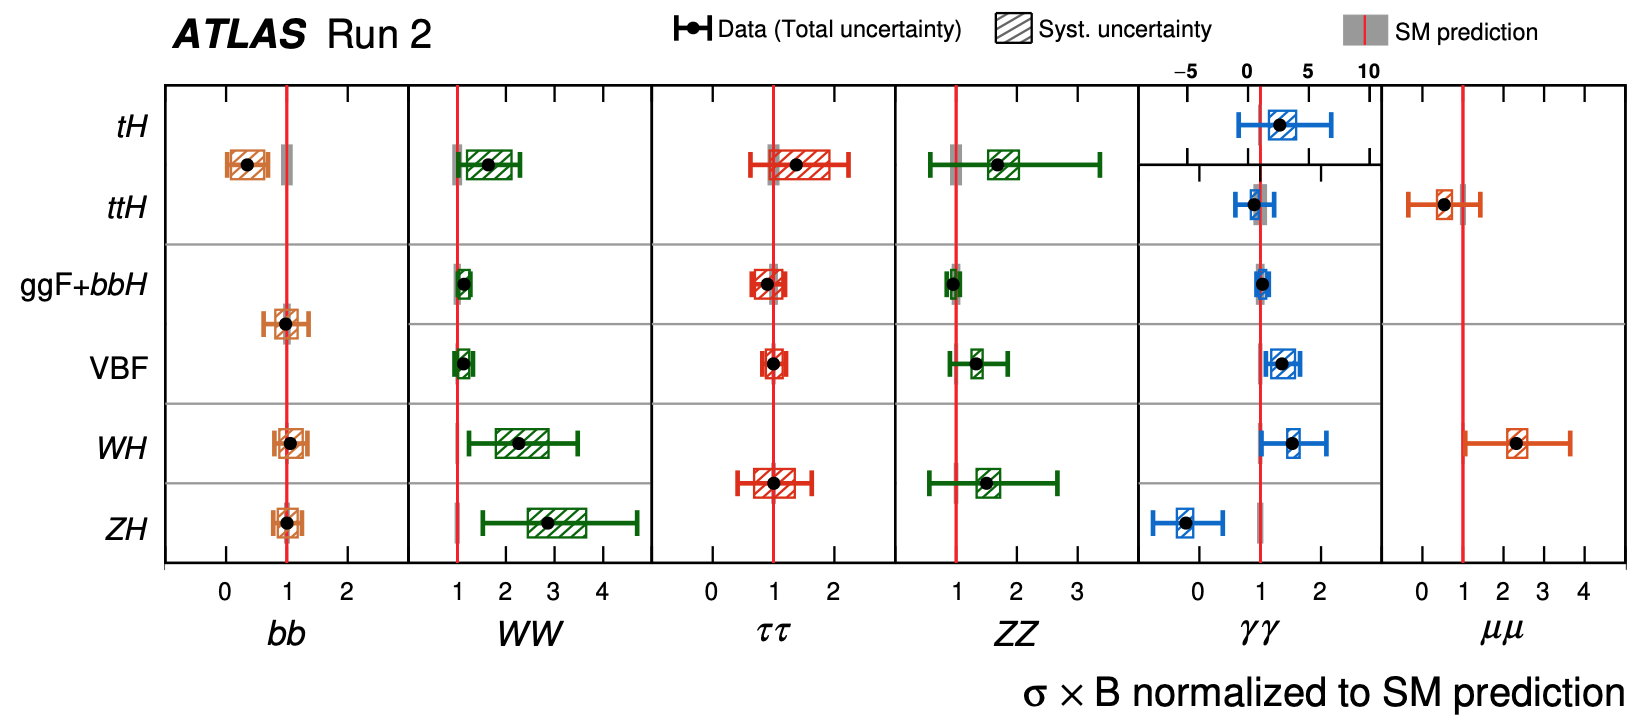
\includegraphics[width=\textwidth]{Images/Theory/allMesRun2.png}
    \caption{Ratio of observed to the SM predicted event rate for different combinations of Higgs boson production and decay mode, from \cite{ATLAS:2022vkf}. The horizontal bars denote the 68\% confidence interval, with grey bands showing the theory uncertainties on the SM cross-section $\times$ branching ratio predictions.}
    \label{fig:measprodH}
\end{figure}

The $W^+W^-$ and $ZZ$ decays can only be achieved by a virtual off-shell Higgs bosons. The fermionic decays are hard to observe due to the larger multi-jet background in a hadron collider. The vector bosons and di-photons leptonic decays benefit from advantageous experimental conditions, being easier to identify thanks to the presence of leptons and suffering from less background contamination. For these reasons, the ATLAS and CMS experiment both observed a particle of mass $m_H = 125$ GeV with the same properties as the Higgs boson in 2012 by combining the $H \rightarrow \gamma\gamma$, $H \rightarrow ZZ \rightarrow \ell^+\ell^-\ell'^+\ell'^-$, and $H \rightarrow W^+W^- \rightarrow \ell^+\ell^-\nu \bar{\nu}$ channels \cite{ATLAS:2012yve, CMS:2012qbp}. This opened the way to many additional Higgs measurements, with some of the most sensitive ones summarised in Figure \ref{fig:measprodH}. Decay modes to third generations particles ($t, b, \tau$) have been observed, with the sensitivity rising for the second generation ($\mu$). In all analyses, the Higgs boson is measured to be in remarkably consistent with the predictions from the \gls{sm} \cite{ATLAS:2022vkf}. 
